\section{Session1 Introduction}
\subsection{Basic of Probability Theory}
\subsubsection{Variables}

\begin{itemize}
    \item (Discrete Random Variable)
    $\mathbb{P}(X = x_i) = p_i, i = 1,2,\cdots,n$
    \item (Continuous Random Variable)
    $\mathbb{P}(r_1<X<r_2) = p$
\end{itemize}

\subsubsection{Probability Density Functions(PDF)}
For the probability $p$ of $X$ lying between $r_1$ and $r_2$, we define the probability density function $f(x)$ as follows:
\[
    \int_{r_1}^{r_2}f(x)dx = p    
\]
\subsubsection{Cumulative Distribution Functions(CDF)}
Let f(x) be the CDF. A cumulative distribution function $F(a)$ tells us probability of a random variable $X$ being less than a certain value $a$:
\[
F(a) = \int_{-\infty}^a f(x)dx = \mathbb{P}(X\leq a)
\]

For CDF, we have following properties:
\begin{itemize}
    \item $f(x)=\frac{dF(x)}{dx}$
    \item $\mathbb{P}(a<X\leq b) = \int_a^bf(x)dx = F(b)-F(a)$
    \item $\mathbb{P}(X>a)=1-F(a)$
\end{itemize}

\subsubsection{Inverse Cumulative Distribution Functions}
Let $F(a)$ be the cumulative distribution function. We define the inverse function $F^{-1}(p)$, the inverse cumulative distribution, as follows:
\[
    F^{-1}(p) = a
\]

The inverse distribution function is also called the \textbf{quantile function}.

The inverse distribution function has following properties:

\begin{itemize}
    \item $F^{-1}(p)$ is non-decreasing.
    \item $F^{-1}(y) \leq x $ if and only if $y\leq F(x)$.
    \item If $Y$ has a uniform distribution in the interval $[0, 1]$, then $F^{-1}(Y)$ is a random variable with distribution $F$.
    \begin{remark}
    If Y has a uniform distribution in the interval $[0, 1]$, we get $F(Y) = Y$, then $F^{-1}(Y) = Y$.
    \end{remark}
\end{itemize}

\subsubsection{Mutually Exclusive Events}

For a given random variable, the probability of any of two mutually exclusive events A and B occurring is just the sum of their individual probabilities.
\[
\mathbb{P}(A\cup B) = \mathbb{P}{(A)} + \mathbb{P}{(B)}    
\]

\subsubsection{Independent Events and Joint Probability}

If the outcome of one random variable is not influenced by the outcome of the other random variable, then we say those variables are independent. The joint probability of $A$ and $B$ is such that
\[
\mathbb{P}(A\cap B) = \mathbb{P}{(A)} \mathbb{P}{(B)}    
\]

\subsubsection{Probability Matrices}
When dealing with the joint probabilities of two variables, it is often convenient to summarize the various probabilities in a probability matrix or probability table.

\begin{example}
\begin{figure}[!ht]
	\centering
	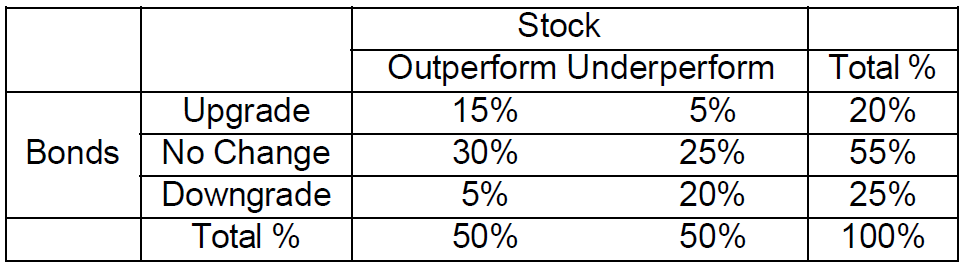
\includegraphics[width=\textwidth]{probability_matrix.png}
	\caption{Stock Grading by Equity Analyst and Credit Rating
    Agency}
\end{figure}
\end{example}

\subsubsection{Conditional Probability}
Probability of A given that B is:
\[
\mathbb{P}(A|B) = \frac{\mathbb{P}(AB)}{\mathbb{P}(B)}
\]

If $\mathbb{P}(A|B) = \mathbb{P}(A)$ , the two random variables $A$ and $B$, are independent.

\subsection{Bayesian Analysis}
\subsubsection{Definition}
For two random variables, $A$ and $B$, Bayes’ theorem states that
\[
    \mathbb{P}(A|B) = \frac{\mathbb{P}(B|A)\mathbb{P}(A)}{\mathbb{P}(B)}
\]

\begin{remark}
    To see sample problems, go for QF603session1 pdf from page45 to page68.
\end{remark}
